\documentclass{article}
\usepackage{graphicx}
\title{Happywhale - Whale and Dolphin Identification}
\author{Matthew Harding}
\date{April 2024}

\begin{document}
\maketitle

\section{Introduction}
This project explores the problem of classifiying images of dolphin and whales to identify indivduals. This work 
is based on the \emph{Happywhale - Whale and Dolphin Identification} Kaggle competition.\par

Data for this competition contains images of over 15,000 unique individual marine mammals from 30 different species collected from 28 different research organizations. 
Individuals have been manually identified and given an individual\_id by marine researches.\par

Unlike a typical classification problem in which there is a fixed set of classes which examples of all classes within the training data, this problem required the ability to classify individuals not contained within the training dataset.

\section{Training Data}

\begin{figure}
    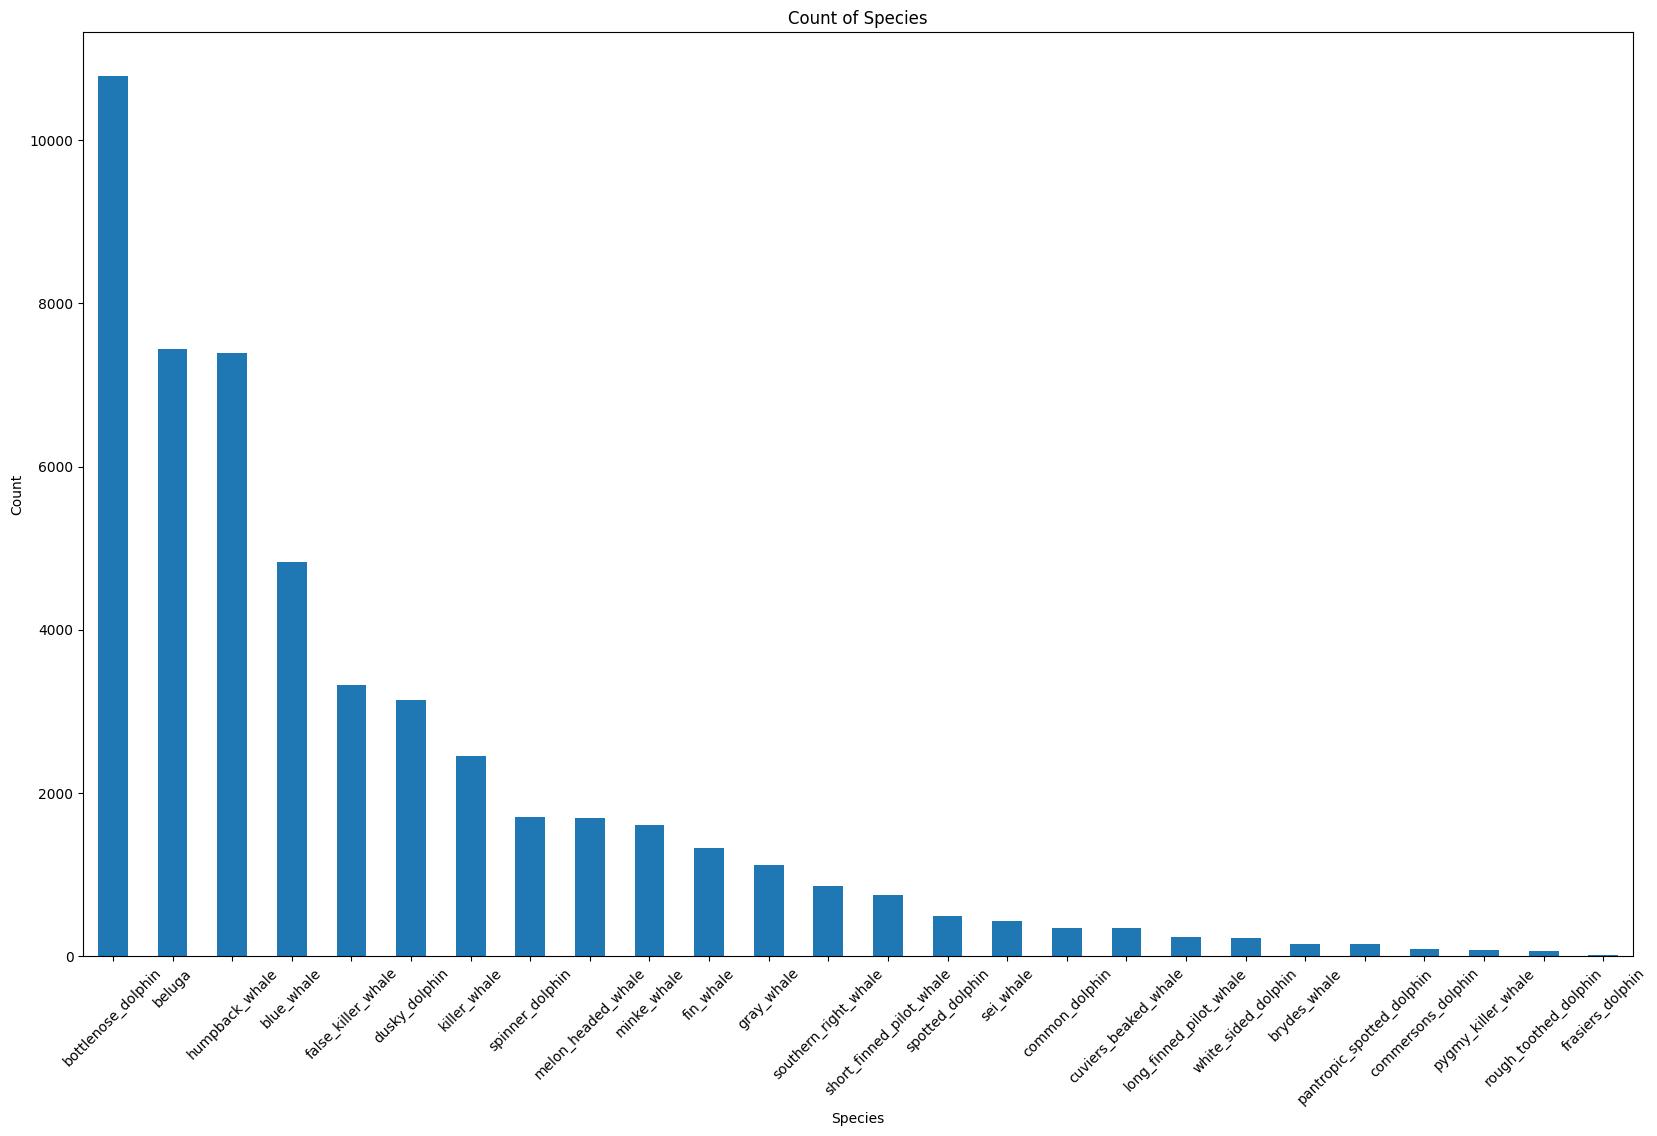
\includegraphics[width=\linewidth]{species_histogram.png}
    \caption{Number of training images per species}
    \label{fig:species_count_histogram}
\end{figure}

\begin{figure}
    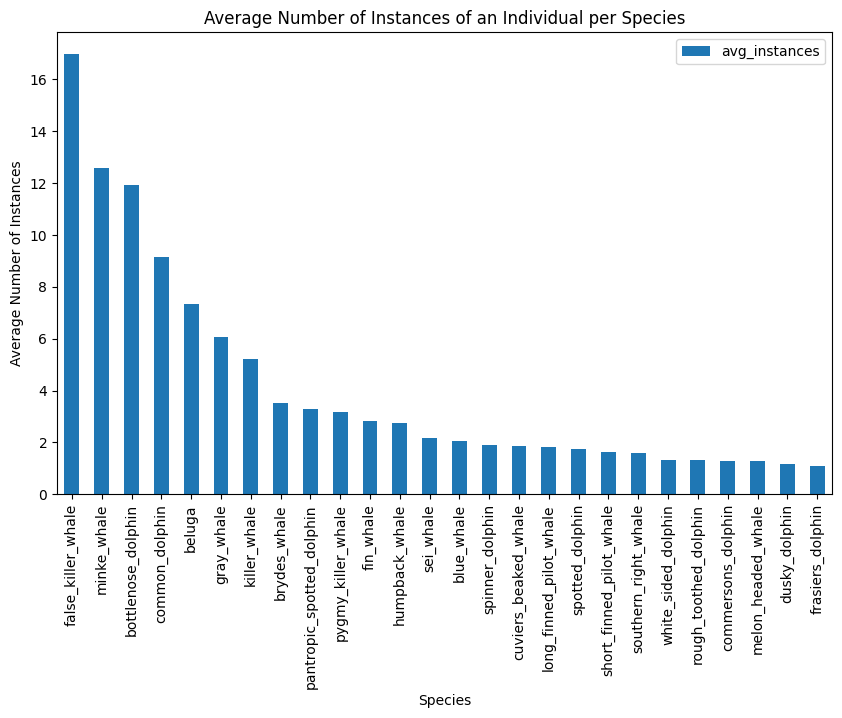
\includegraphics[width=\linewidth]{mean_individuals_histogram.png}
    \caption{Mean count of images per individual by species}
    \label{fig:individual_mean_count_histogram}
\end{figure}

Within the training data there are 51,033 labelled images. Looking at the histogram of species Figure \ref{fig:species_count_histogram}, there is a clear inbalance in the number of iamges per species with the vast majority
of labelled images being for bottlenose dolphins, beluga whales, humpback whales and blue whales. For some species the number of examples it so low it will be difficult to gain a high level of accuracy within classification.

Look at Figure \ref{fig:individual_mean_count_histogram}, the mean count of images per indivdual by species we see another imbalance with some species on average containing a large number of images per indivudal whilst others only contain one or two images per individual.

Given these issues with the dataset combined in compute limitations, it was decided to limit the task to building a classify for bottlenose dolphins, a species for which there were a large number of labelled images and for which there 
were on average a large number of images per individual. By doing this, the total training dataset was reduced to 9664 images across 613 individuals.

\section{Image Preprocessing}

The training images for the bottlenose dolphins came in a variety of sizes. Figure \ref{example_train} shows an example unprocessed image. Large amounts of each image are just of water which is irrelvant to the classification task. We are only interested in the parts of the 
images that contain the animals.

A solution to this issue was proposed within the discussions of the Kaggle competition. YoloV5 was trained on a dataset of 1200 pictures of whale flukes and the corresponding location of points on the edge of the fluke for those pictures. 
This was then assumed to generalise to finding the bounding box for any part of a whale or dolphin within the water. However, it is worth noting that finding the bounding box of any part of the animal is considered an Out of Distribution problem. 

From this technique a cropped dataset was created with all images having a dimension of 256 x 256. 


https://www.kaggle.com/datasets/martinpiotte/humpback-whale-identification-fluke-location
https://www.kaggle.com/code/awsaf49/happywhale-cropped-data-prepare-yolov5





\begin{figure}
    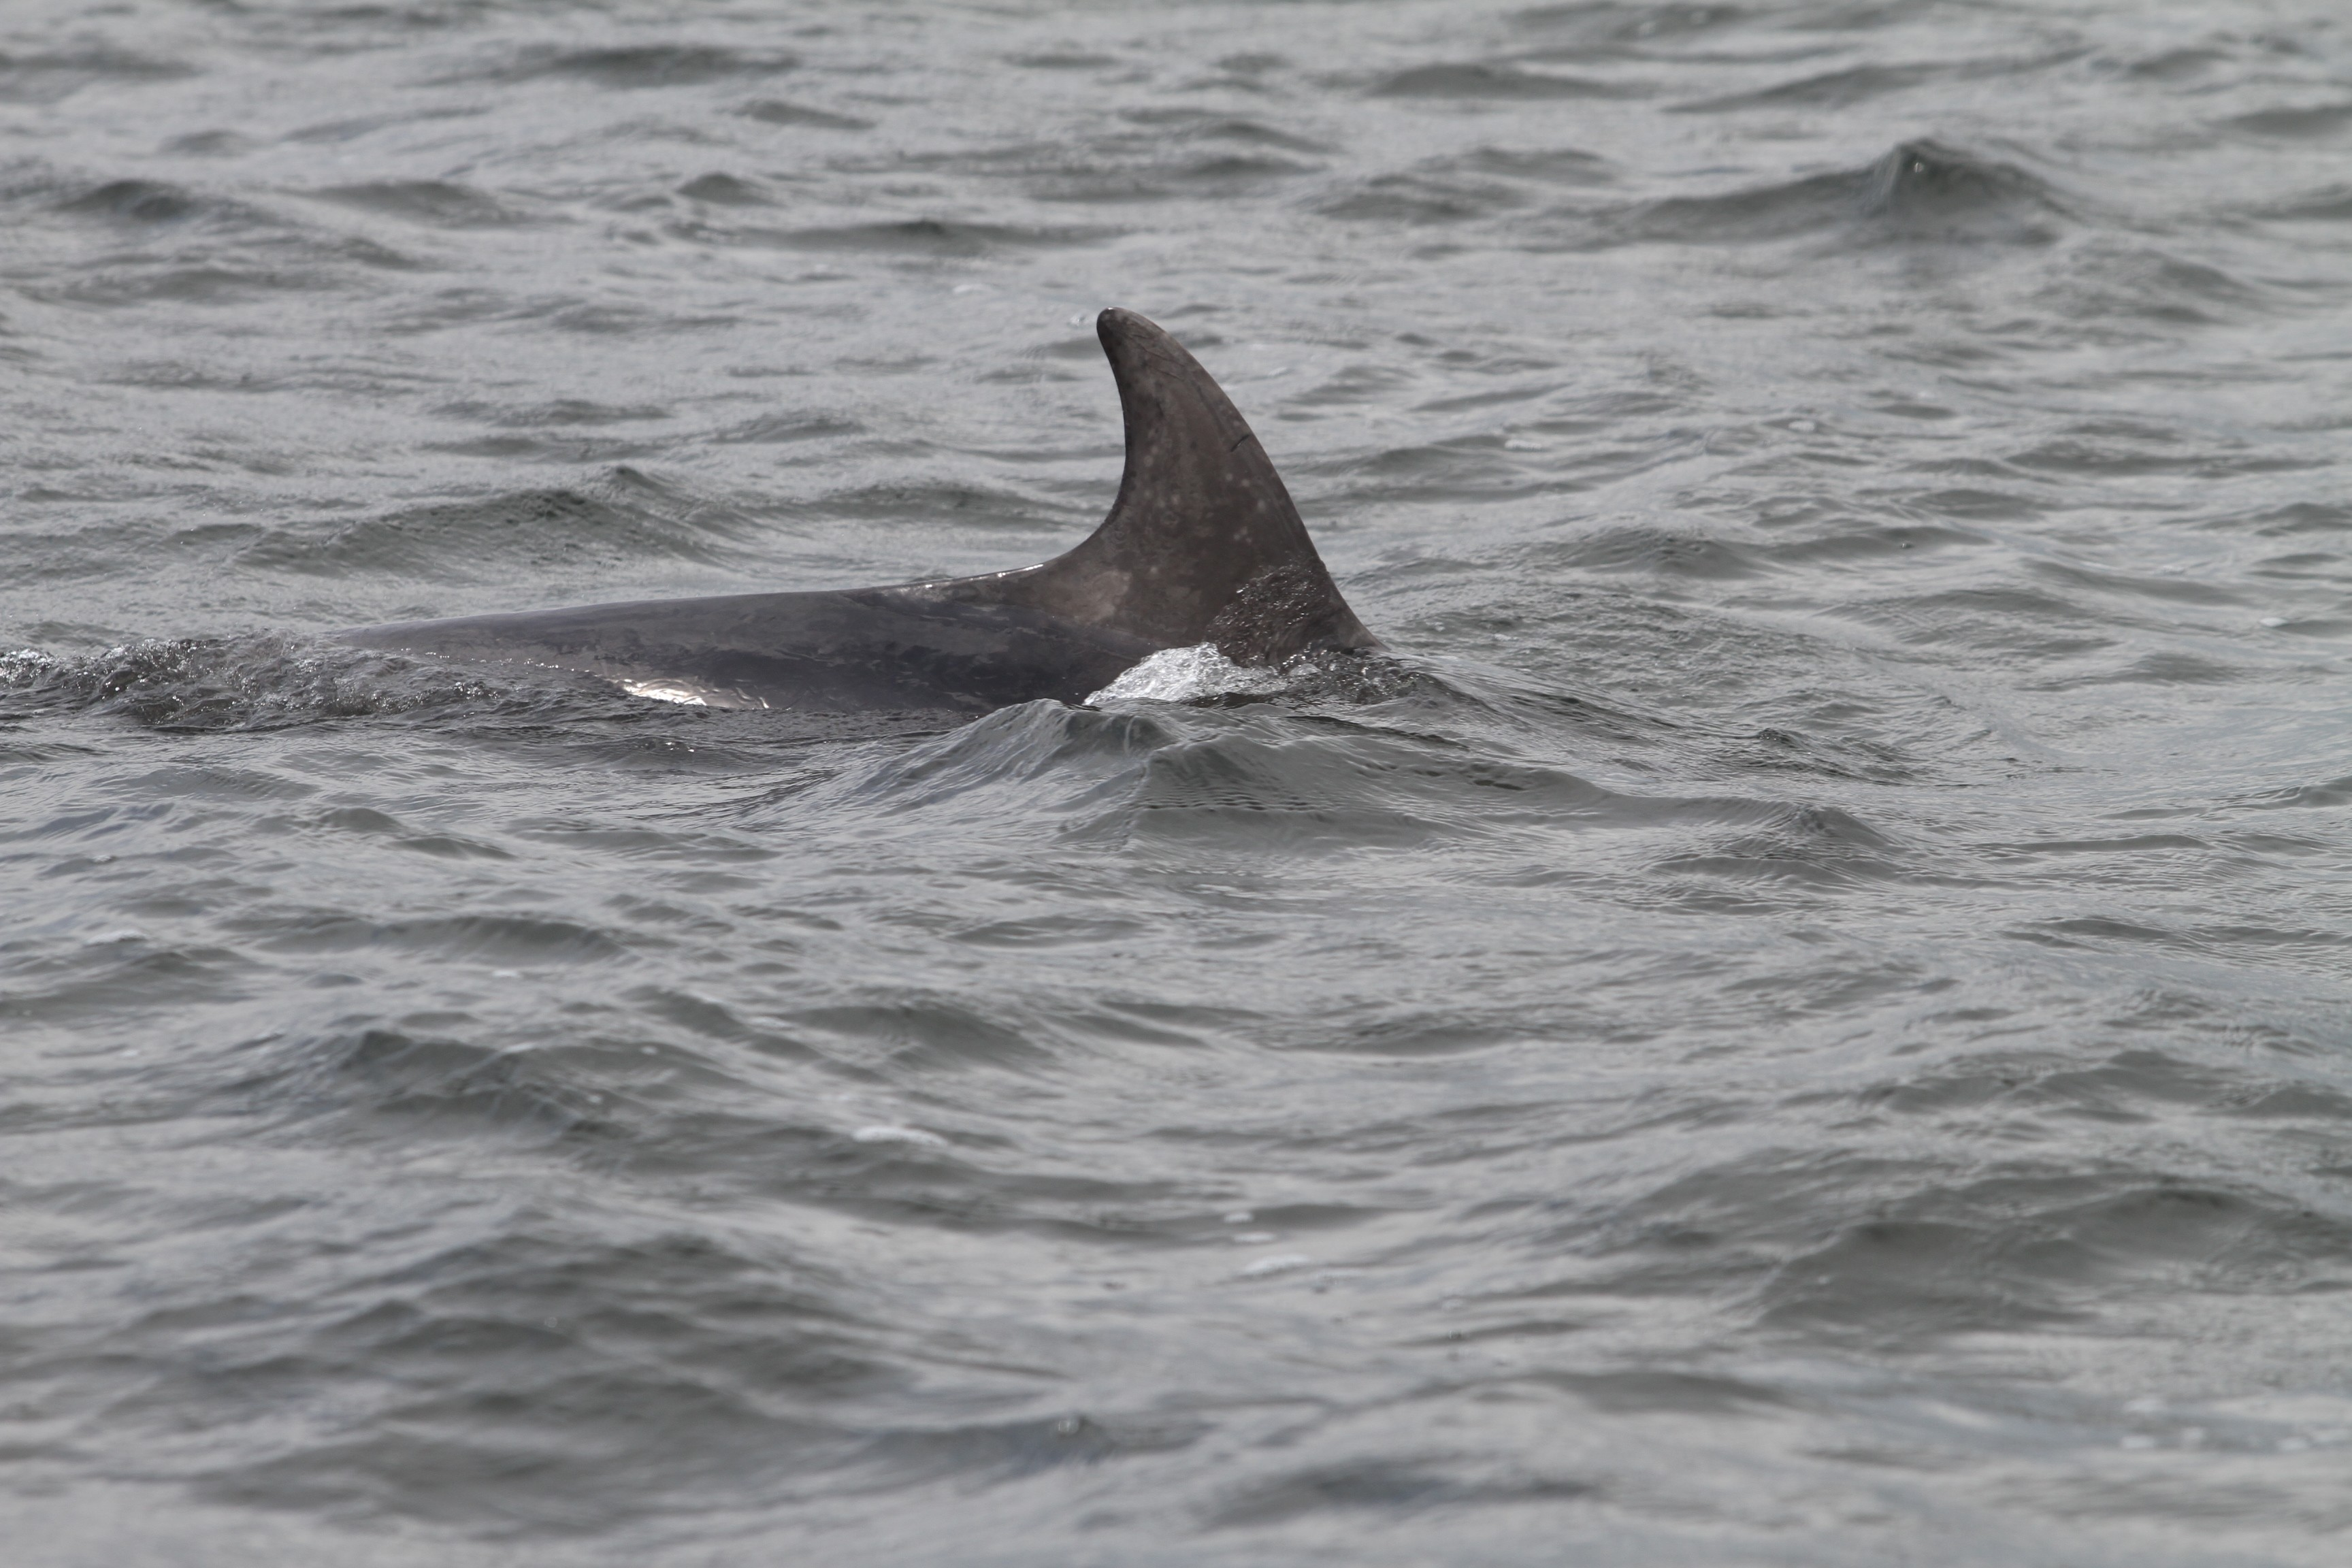
\includegraphics[width=\linewidth]{example_train.jpg}
    \caption{Example image of a bottlenose dolphin}
    \label{fig:example_train}
\end{figure}

\section{Measuring Model Performance}

Performance of the model was measured via the Mean Average Precision @ 5 (MAP@5). Instead of using just accuracy as a measure, MAP@5 was used to account of the complexity of the
classification task. Accuracy only considers whether the top predicted class is correct or not. It does not take into account the ranking of predictions. MAP@5, on the other hand, considers the ranking of predictions within the top 5 predicted classes. It rewards models that rank the correct classes higher in the prediction list.




\section{Model Training}

Despite the massive reduction in file size that came from using the cropped dataset instead of the original dataset, training times on the local machine was still prohibitively long. Therefore, training was done using AWS Sagemaker.

The first approach taken was to classify images

\end{document}